\documentclass[12pt,a4paper]{article}\usepackage[]{graphicx}\usepackage[]{color}
% maxwidth is the original width if it is less than linewidth
% otherwise use linewidth (to make sure the graphics do not exceed the margin)
\makeatletter
\def\maxwidth{ %
  \ifdim\Gin@nat@width>\linewidth
    \linewidth
  \else
    \Gin@nat@width
  \fi
}
\makeatother

\definecolor{fgcolor}{rgb}{0.345, 0.345, 0.345}
\newcommand{\hlnum}[1]{\textcolor[rgb]{0.686,0.059,0.569}{#1}}%
\newcommand{\hlstr}[1]{\textcolor[rgb]{0.192,0.494,0.8}{#1}}%
\newcommand{\hlcom}[1]{\textcolor[rgb]{0.678,0.584,0.686}{\textit{#1}}}%
\newcommand{\hlopt}[1]{\textcolor[rgb]{0,0,0}{#1}}%
\newcommand{\hlstd}[1]{\textcolor[rgb]{0.345,0.345,0.345}{#1}}%
\newcommand{\hlkwa}[1]{\textcolor[rgb]{0.161,0.373,0.58}{\textbf{#1}}}%
\newcommand{\hlkwb}[1]{\textcolor[rgb]{0.69,0.353,0.396}{#1}}%
\newcommand{\hlkwc}[1]{\textcolor[rgb]{0.333,0.667,0.333}{#1}}%
\newcommand{\hlkwd}[1]{\textcolor[rgb]{0.737,0.353,0.396}{\textbf{#1}}}%
\let\hlipl\hlkwb

\usepackage{framed}
\makeatletter
\newenvironment{kframe}{%
 \def\at@end@of@kframe{}%
 \ifinner\ifhmode%
  \def\at@end@of@kframe{\end{minipage}}%
  \begin{minipage}{\columnwidth}%
 \fi\fi%
 \def\FrameCommand##1{\hskip\@totalleftmargin \hskip-\fboxsep
 \colorbox{shadecolor}{##1}\hskip-\fboxsep
     % There is no \\@totalrightmargin, so:
     \hskip-\linewidth \hskip-\@totalleftmargin \hskip\columnwidth}%
 \MakeFramed {\advance\hsize-\width
   \@totalleftmargin\z@ \linewidth\hsize
   \@setminipage}}%
 {\par\unskip\endMakeFramed%
 \at@end@of@kframe}
\makeatother

\definecolor{shadecolor}{rgb}{.97, .97, .97}
\definecolor{messagecolor}{rgb}{0, 0, 0}
\definecolor{warningcolor}{rgb}{1, 0, 1}
\definecolor{errorcolor}{rgb}{1, 0, 0}
\newenvironment{knitrout}{}{} % an empty environment to be redefined in TeX

\usepackage{alltt}

\usepackage{amsfonts}
\usepackage{amsmath}
\usepackage{hyperref}
%\usepackage[backend=biber,sorting=none]{biblatex}

%\bibliography{BIBLIOGRAPHY}

\author{James Foadi \\ 
        email \href{mailto:j.foadi@bath.ac.uk}{j.foadi@bath.ac.uk}}
\date{June, 2019}

\title{Tutorial 1: Play with thiocyanate}

%\VignetteIndexEntry{Play with thiocyanate}
%\VignetteEngine{knitr::knitr}

%<<setup, eval= TRUE, include= FALSE, cache= FALSE, echo= FALSE>>=
%system ("biber tutorial01")
%@
\IfFileExists{upquote.sty}{\usepackage{upquote}}{}
\begin{document}

\maketitle

\noindent Main aim of this tutorial is to get you rapidly acquainted with some of the most common and useful functions of the package \texttt{crone}.

\section{Load data related to the structure}
There are two types of data related to each 1D structure, the `direct-space' data and the `reciprocal-space' data. The first type of data include the position of each atom in the structure, its B factor (a measure of the thermal vibration of the atom) and the occupancy (which essentially describes what fraction of the specific atom is contained in each unit cell). Part of these data are also the unit cell's length, $a$, and the type of symmetry (only $P1$ or $P\bar{1}$ for 1D structures). The second type of data include experimental data related to the structure, i.e. data due to the x-ray diffraction of the structure itself. These data are not always the same, but should at least consist of the Miller index $h$ and of the observed amplitudes of the structure factors and their experimental errors. The first type of data are known as \emph{sdata}, while the second type are known as \emph{fdata}. Both types are R named lists.\\
\newline
\noindent The function responsible to load an \texttt{sdata} object is \texttt{load\_structure}. If called without argument, this function returns all the structures included in \texttt{crone}'s internal library of structures:

\begin{small}
\begin{knitrout}
\definecolor{shadecolor}{rgb}{0.969, 0.969, 0.969}\color{fgcolor}\begin{kframe}
\begin{alltt}
\hlkwd{library}\hlstd{(crone)}
\hlkwd{load_structure}\hlstd{()}
\end{alltt}


{\ttfamily\noindent\itshape\color{messagecolor}{\#\# \\\#\# 1D structures available for loading:}}

{\ttfamily\noindent\itshape\color{messagecolor}{\#\#\ \ \ \ beryllium\_fluoride}}

{\ttfamily\noindent\itshape\color{messagecolor}{\#\#\ \ \ \ carbon\_dioxide}}

{\ttfamily\noindent\itshape\color{messagecolor}{\#\#\ \ \ \ cyanate}}

{\ttfamily\noindent\itshape\color{messagecolor}{\#\#\ \ \ \ nitronium}}

{\ttfamily\noindent\itshape\color{messagecolor}{\#\#\ \ \ \ thiocyanate}}

{\ttfamily\noindent\itshape\color{messagecolor}{\#\#\ \ \ \ xenon\_difluoride}}

{\ttfamily\noindent\itshape\color{messagecolor}{\#\#\ \ \ \ pinkerton2015}}

{\ttfamily\noindent\itshape\color{messagecolor}{\#\# Please use an appropriate name - e.g. load\_structure("{}cyanate"{})}}\end{kframe}
\end{knitrout}
\end{small}

\noindent Let's try and load data corresponding to thiocyanate:

\begin{knitrout}
\definecolor{shadecolor}{rgb}{0.969, 0.969, 0.969}\color{fgcolor}\begin{kframe}
\begin{alltt}
\hlcom{# Make sure to type the underscore!}
\hlstd{sdata} \hlkwb{<-} \hlkwd{load_structure}\hlstd{(}\hlstr{"thiocyanate"}\hlstd{)}

\hlcom{# The object returned by load_structure is a named list}
\hlkwd{class}\hlstd{(sdata)}
\end{alltt}
\begin{verbatim}
## [1] "list"
\end{verbatim}
\begin{alltt}
\hlkwd{names}\hlstd{(sdata)}
\end{alltt}
\begin{verbatim}
## [1] "a"   "SG"  "x0"  "Z"   "B"   "occ"
\end{verbatim}
\end{kframe}
\end{knitrout}

\noindent \texttt{a} and \texttt{SG}, as said before, are the unit cell's length (in angstroms) and space group symbol, respectively:

\begin{knitrout}
\definecolor{shadecolor}{rgb}{0.969, 0.969, 0.969}\color{fgcolor}\begin{kframe}
\begin{alltt}
\hlstd{sdata}\hlopt{$}\hlstd{a}
\end{alltt}
\begin{verbatim}
## [1] 4.969
\end{verbatim}
\begin{alltt}
\hlstd{sdata}\hlopt{$}\hlstd{SG}
\end{alltt}
\begin{verbatim}
## [1] "P1"
\end{verbatim}
\end{kframe}
\end{knitrout}

\noindent The next four elements of the list are vectors of equal length, each one containing the rest position of the atom, the corresponding atomic number, the B factor and the occupancy:

\begin{knitrout}
\definecolor{shadecolor}{rgb}{0.969, 0.969, 0.969}\color{fgcolor}\begin{kframe}
\begin{alltt}
\hlstd{sdata}\hlopt{$}\hlstd{x0}
\end{alltt}
\begin{verbatim}
## [1] 1.000 2.813 3.969
\end{verbatim}
\begin{alltt}
\hlstd{sdata}\hlopt{$}\hlstd{Z}
\end{alltt}
\begin{verbatim}
## [1] 16  6  7
\end{verbatim}
\begin{alltt}
\hlstd{sdata}\hlopt{$}\hlstd{B}
\end{alltt}
\begin{verbatim}
## [1]  5.000 13.333 11.429
\end{verbatim}
\begin{alltt}
\hlstd{sdata}\hlopt{$}\hlstd{occ}
\end{alltt}
\begin{verbatim}
## [1] 1 1 1
\end{verbatim}
\end{kframe}
\end{knitrout}

\noindent Thus, we have a sulphur (Z=16) at position $x=1$ in the cell, a carbon (Z=6) at $x=2.813$ and a nitrogen (Z=7) at $x=3.969$. The sulphur, being the heaviest element, vibrates less than the nitrogen (smaller B factor), which vibrates less than the carbon. Also, each one of these atoms is fully present in all unit cells of the 1D crystal.

\section{Calculate and plot the structure}
\noindent The actual electron density $\rho(x)$ of this structure can be calculated using the function \texttt{structure\_gauss}. This can be then plotted to show the extent of the structure. Coloured discs corresponding to the accepted colour coding for chemical elements can be added in the bottom part of the plot, at the exact locations of the atomic centres:

\begin{center}
\begin{knitrout}
\definecolor{shadecolor}{rgb}{0.969, 0.969, 0.969}\color{fgcolor}\begin{kframe}
\begin{alltt}
\hlstd{rtmp} \hlkwb{<-} \hlkwd{structure_gauss}\hlstd{(sdata)}
\hlkwd{names}\hlstd{(rtmp)}
\end{alltt}
\begin{verbatim}
## [1] "x"  "rr"
\end{verbatim}
\begin{alltt}
\hlkwd{plot}\hlstd{(rtmp}\hlopt{$}\hlstd{x,rtmp}\hlopt{$}\hlstd{rr,}\hlkwc{type}\hlstd{=}\hlstr{"l"}\hlstd{,}\hlkwc{xlab}\hlstd{=}\hlstr{"x"}\hlstd{,}\hlkwc{ylab}\hlstd{=}\hlkwd{expression}\hlstd{(rho),}
     \hlkwc{ylim}\hlstd{=}\hlkwd{c}\hlstd{(}\hlopt{-}\hlnum{1}\hlstd{,}\hlkwd{max}\hlstd{(rtmp}\hlopt{$}\hlstd{rr)))}
\hlkwd{segments}\hlstd{(sdata}\hlopt{$}\hlstd{x[}\hlnum{1}\hlstd{],}\hlnum{0}\hlstd{,sdata}\hlopt{$}\hlstd{x[}\hlnum{3}\hlstd{],}\hlnum{0}\hlstd{,}\hlkwc{lwd}\hlstd{=}\hlnum{2}\hlstd{)}
\hlkwd{points}\hlstd{(sdata}\hlopt{$}\hlstd{x[}\hlnum{1}\hlstd{],}\hlnum{0}\hlstd{,}\hlkwc{pch}\hlstd{=}\hlnum{16}\hlstd{,}\hlkwc{cex}\hlstd{=}\hlnum{3}\hlstd{,}\hlkwc{col}\hlstd{=}\hlstr{"yellow"}\hlstd{)}
\hlkwd{points}\hlstd{(sdata}\hlopt{$}\hlstd{x[}\hlnum{2}\hlstd{],}\hlnum{0}\hlstd{,}\hlkwc{pch}\hlstd{=}\hlnum{16}\hlstd{,}\hlkwc{cex}\hlstd{=}\hlnum{3}\hlstd{,}\hlkwc{col}\hlstd{=}\hlstr{"grey"}\hlstd{)}
\hlkwd{points}\hlstd{(sdata}\hlopt{$}\hlstd{x[}\hlnum{3}\hlstd{],}\hlnum{0}\hlstd{,}\hlkwc{pch}\hlstd{=}\hlnum{16}\hlstd{,}\hlkwc{cex}\hlstd{=}\hlnum{3}\hlstd{,}\hlkwc{col}\hlstd{=}\hlstr{"blue"}\hlstd{)}
\end{alltt}
\end{kframe}
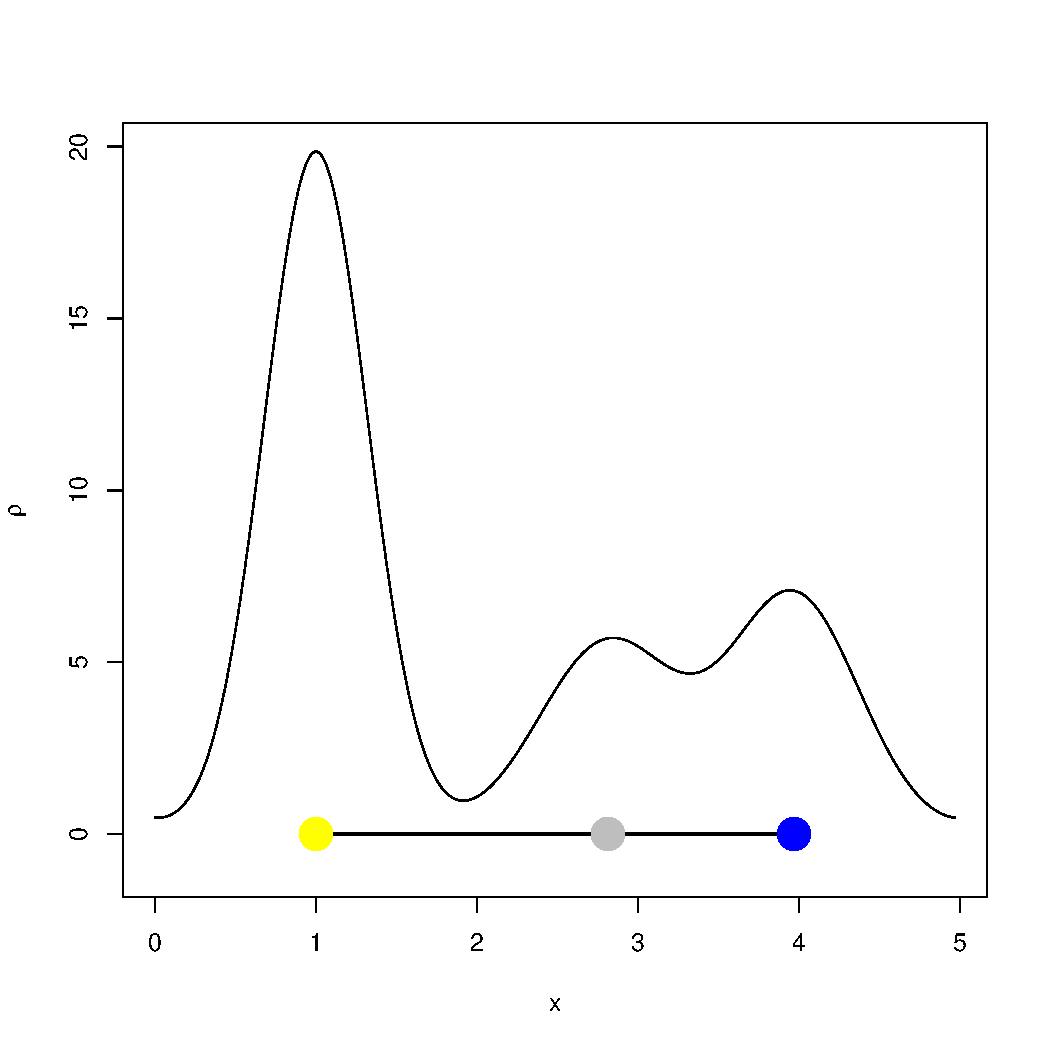
\includegraphics[width=3.2in]{figure/ch05-1} 

\end{knitrout}
\end{center}

\noindent In fact, a grid containing several adjacent unit cells can be provided to the function \texttt{structure\_gauss} so that the extent of the crystal periodicity is displayed. For 10 contiguous cells we have, for instance:

\begin{center}
\begin{knitrout}
\definecolor{shadecolor}{rgb}{0.969, 0.969, 0.969}\color{fgcolor}\begin{kframe}
\begin{alltt}
\hlstd{x} \hlkwb{<-} \hlkwd{seq}\hlstd{(}\hlnum{0}\hlstd{,}\hlnum{10}\hlopt{*}\hlstd{sdata}\hlopt{$}\hlstd{a,}\hlkwc{length}\hlstd{=}\hlnum{1000}\hlstd{)}
\hlstd{rtmp} \hlkwb{<-} \hlkwd{structure_gauss}\hlstd{(sdata,x)}
\hlkwd{plot}\hlstd{(rtmp}\hlopt{$}\hlstd{x,rtmp}\hlopt{$}\hlstd{rr,}\hlkwc{type}\hlstd{=}\hlstr{"l"}\hlstd{,}\hlkwc{xlab}\hlstd{=}\hlstr{"x"}\hlstd{,}\hlkwc{ylab}\hlstd{=}\hlkwd{expression}\hlstd{(rho))}
\end{alltt}
\end{kframe}
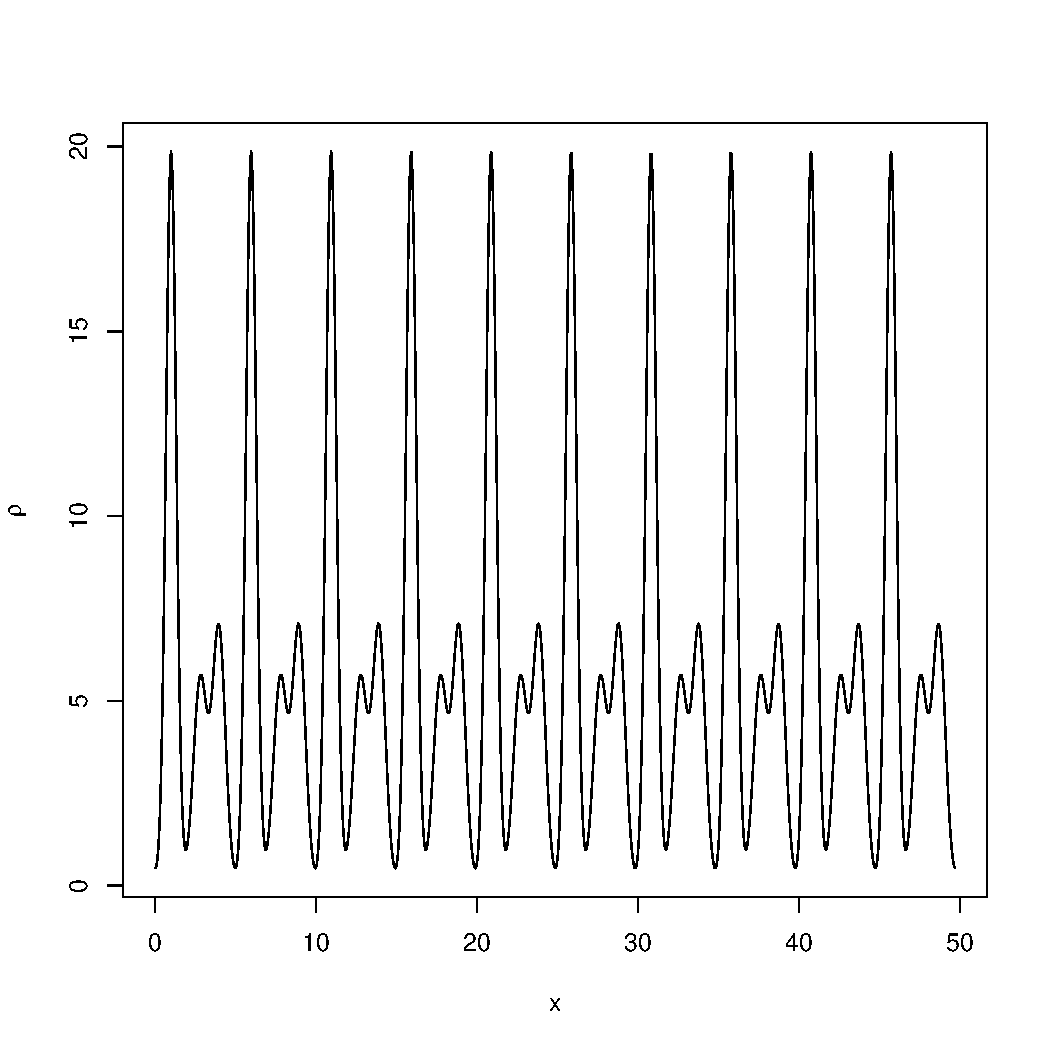
\includegraphics[width=3.2in]{figure/ch06-1} 

\end{knitrout}
\end{center}

\section{The calculation of structure factors}
\noindent The product of a diffraction process are intensities whose square roots are, essentially, the amplitudes of the structure factors, $| F_h |$. Amplitudes and phases related to the given structure can be calculated using the function \texttt{strufac}. Structure factors will be computed for every value of the Miller indices provided:

\begin{knitrout}
\definecolor{shadecolor}{rgb}{0.969, 0.969, 0.969}\color{fgcolor}\begin{kframe}
\begin{alltt}
\hlstd{hidx} \hlkwb{<-} \hlkwd{c}\hlstd{(}\hlnum{0}\hlstd{,}\hlnum{1}\hlstd{)}
\hlstd{ftmp} \hlkwb{<-} \hlkwd{strufac}\hlstd{(hidx,sdata)}
\hlkwd{names}\hlstd{(ftmp)}
\end{alltt}
\begin{verbatim}
## [1] "Fmod" "Fpha"
\end{verbatim}
\begin{alltt}
\hlstd{ftmp}\hlopt{$}\hlstd{Fmod}  \hlcom{# Structure factors' amplitudes for h=0,1}
\end{alltt}
\begin{verbatim}
## [1] 29.000000  6.289007
\end{verbatim}
\begin{alltt}
\hlstd{ftmp}\hlopt{$}\hlstd{Fpha}  \hlcom{# Structure factors' phases for h=0,1}
\end{alltt}
\begin{verbatim}
## [1]  0.00000 75.66567
\end{verbatim}
\begin{alltt}
\hlstd{hidx} \hlkwb{=} \hlopt{-}\hlnum{2}\hlopt{:}\hlnum{2}
\hlstd{ftmp} \hlkwb{<-} \hlkwd{strufac}\hlstd{(hidx,sdata)}
\hlstd{ftmp}\hlopt{$}\hlstd{Fmod}  \hlcom{# Friedel's law |F(-h)|=|F(h)|}
\end{alltt}
\begin{verbatim}
## [1] 12.500798  6.289007 29.000000  6.289007 12.500798
\end{verbatim}
\begin{alltt}
\hlstd{ftmp}\hlopt{$}\hlstd{Fpha}  \hlcom{# Friedel's law phi(-h)=-phi(h)}
\end{alltt}
\begin{verbatim}
## [1] -147.71590  -75.66567    0.00000   75.66567  147.71590
\end{verbatim}
\end{kframe}
\end{knitrout}

\section{Electron density as Fourier synthesis}
\noindent The electron density can be recovered starting from the experimental data (the structure factors' amplitudes) and the structure factors' phases, if these are known. The calculation is known as Fourier synthesis
\begin{equation*}
\rho(x) = \frac{1}{a}| F_0 | + \frac{2}{a}\sum_{h=1}^{h_{\mathrm{max}}} | F_h |\cos\left(2\pi h\frac{x}{a}\right),
\end{equation*}
and it is carried out by the function \texttt{fousynth}. The input for this function are the available indices, the corresponding amplitudes and phases of the structure factors, the unit cell length and the number of points for the regular grid used to calculate the electron density. In the following example let's calculate the approximated electron density using 2,3,5, 10 Fourier components, and compare it with the exact analytic density.

\begin{center}
\begin{knitrout}
\definecolor{shadecolor}{rgb}{0.969, 0.969, 0.969}\color{fgcolor}\begin{kframe}
\begin{alltt}
\hlstd{hidx} \hlkwb{<-} \hlnum{0}\hlopt{:}\hlnum{10}
\hlstd{ftmp} \hlkwb{<-} \hlkwd{strufac}\hlstd{(}\hlkwc{hidx}\hlstd{=hidx,}\hlkwc{sdata}\hlstd{=sdata)}

\hlcom{# Grid}
\hlstd{N} \hlkwb{<-} \hlnum{200}

\hlcom{# Approximation with hmax=2}
\hlstd{Fmod} \hlkwb{<-} \hlstd{ftmp}\hlopt{$}\hlstd{Fmod[}\hlnum{1}\hlopt{:}\hlnum{3}\hlstd{]}
\hlstd{Fpha} \hlkwb{<-} \hlstd{ftmp}\hlopt{$}\hlstd{Fpha[}\hlnum{1}\hlopt{:}\hlnum{3}\hlstd{]}
\hlstd{hidx} \hlkwb{<-} \hlnum{0}\hlopt{:}\hlnum{2}
\hlstd{rtmp1} \hlkwb{<-} \hlkwd{fousynth}\hlstd{(sdata}\hlopt{$}\hlstd{a,Fmod,Fpha,hidx,N)}

\hlcom{# Approximation with hmax=3}
\hlstd{Fmod} \hlkwb{<-} \hlstd{ftmp}\hlopt{$}\hlstd{Fmod[}\hlnum{1}\hlopt{:}\hlnum{4}\hlstd{]}
\hlstd{Fpha} \hlkwb{<-} \hlstd{ftmp}\hlopt{$}\hlstd{Fpha[}\hlnum{1}\hlopt{:}\hlnum{4}\hlstd{]}
\hlstd{hidx} \hlkwb{<-} \hlnum{0}\hlopt{:}\hlnum{3}
\hlstd{rtmp2} \hlkwb{<-} \hlkwd{fousynth}\hlstd{(sdata}\hlopt{$}\hlstd{a,Fmod,Fpha,hidx,N)}

\hlcom{# Approximation with hmax=5}
\hlstd{Fmod} \hlkwb{<-} \hlstd{ftmp}\hlopt{$}\hlstd{Fmod[}\hlnum{1}\hlopt{:}\hlnum{6}\hlstd{]}
\hlstd{Fpha} \hlkwb{<-} \hlstd{ftmp}\hlopt{$}\hlstd{Fpha[}\hlnum{1}\hlopt{:}\hlnum{6}\hlstd{]}
\hlstd{hidx} \hlkwb{<-} \hlnum{0}\hlopt{:}\hlnum{5}
\hlstd{rtmp3} \hlkwb{<-} \hlkwd{fousynth}\hlstd{(sdata}\hlopt{$}\hlstd{a,Fmod,Fpha,hidx,N)}

\hlcom{# Approximation with hmax=10}
\hlstd{Fmod} \hlkwb{<-} \hlstd{ftmp}\hlopt{$}\hlstd{Fmod[}\hlnum{1}\hlopt{:}\hlnum{11}\hlstd{]}
\hlstd{Fpha} \hlkwb{<-} \hlstd{ftmp}\hlopt{$}\hlstd{Fpha[}\hlnum{1}\hlopt{:}\hlnum{11}\hlstd{]}
\hlstd{hidx} \hlkwb{<-} \hlnum{0}\hlopt{:}\hlnum{10}
\hlstd{rtmp4} \hlkwb{<-} \hlkwd{fousynth}\hlstd{(sdata}\hlopt{$}\hlstd{a,Fmod,Fpha,hidx,N)}

\hlcom{# Limits for plot}
\hlstd{lims} \hlkwb{<-} \hlkwd{range}\hlstd{(rtmp1}\hlopt{$}\hlstd{rr,rtmp2}\hlopt{$}\hlstd{rr,rtmp3}\hlopt{$}\hlstd{rr,rtmp4}\hlopt{$}\hlstd{rr,rtmp}\hlopt{$}\hlstd{rr)}

\hlcom{# Comparisons}
\hlkwd{plot}\hlstd{(rtmp1}\hlopt{$}\hlstd{x,rtmp1}\hlopt{$}\hlstd{rr,}\hlkwc{type}\hlstd{=}\hlstr{"l"}\hlstd{,}\hlkwc{xlab}\hlstd{=}\hlstr{"x"}\hlstd{,}\hlkwc{ylab}\hlstd{=}\hlkwd{expression}\hlstd{(rho),}
     \hlkwc{ylim}\hlstd{=lims)}
\hlkwd{points}\hlstd{(rtmp2}\hlopt{$}\hlstd{x,rtmp2}\hlopt{$}\hlstd{rr,}\hlkwc{type}\hlstd{=}\hlstr{"l"}\hlstd{,}\hlkwc{col}\hlstd{=}\hlnum{2}\hlstd{)}
\hlkwd{points}\hlstd{(rtmp3}\hlopt{$}\hlstd{x,rtmp3}\hlopt{$}\hlstd{rr,}\hlkwc{type}\hlstd{=}\hlstr{"l"}\hlstd{,}\hlkwc{col}\hlstd{=}\hlnum{3}\hlstd{)}
\hlkwd{points}\hlstd{(rtmp4}\hlopt{$}\hlstd{x,rtmp4}\hlopt{$}\hlstd{rr,}\hlkwc{type}\hlstd{=}\hlstr{"l"}\hlstd{,}\hlkwc{col}\hlstd{=}\hlnum{4}\hlstd{)}
\hlkwd{points}\hlstd{(rtmp}\hlopt{$}\hlstd{x,rtmp}\hlopt{$}\hlstd{rr,}\hlkwc{type}\hlstd{=}\hlstr{"l"}\hlstd{,}\hlkwc{col}\hlstd{=}\hlnum{1}\hlstd{,}\hlkwc{lwd}\hlstd{=}\hlnum{3}\hlstd{,}\hlkwc{lty}\hlstd{=}\hlnum{2}\hlstd{)}
\end{alltt}
\end{kframe}
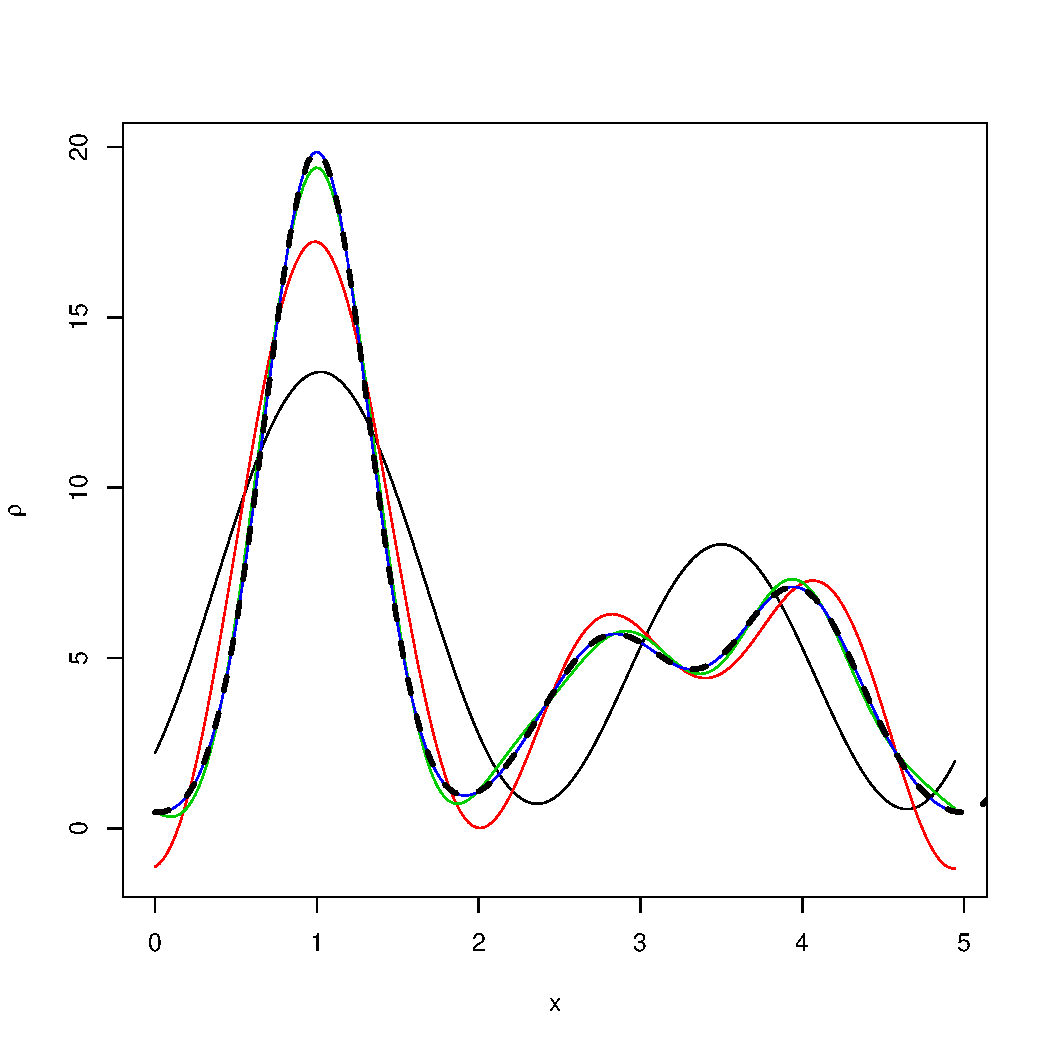
\includegraphics[width=4.5in]{figure/ch08-1} 

\end{knitrout}
\end{center}

\noindent The Fourier synthesis with $h_{\mathrm{max}}=10$ is quite close to the exact analytic density.

\section{Load experimental data}
The structure factors related to a specific structure can be loaded with the function \texttt{load\_data}. This function will produce the \emph{fdata} type. Let's practice with the thiocyanate structure.

\begin{knitrout}
\definecolor{shadecolor}{rgb}{0.969, 0.969, 0.969}\color{fgcolor}\begin{kframe}
\begin{alltt}
\hlstd{fdata} \hlkwb{<-} \hlkwd{load_data}\hlstd{(}\hlkwc{sname}\hlstd{=}\hlstr{"thiocyanate"}\hlstd{)}

\hlcom{# Names of fdata elements}
\hlstd{ntmp} \hlkwb{<-} \hlkwd{names}\hlstd{(fdata)}
\hlkwa{for} \hlstd{(a} \hlkwa{in} \hlstd{ntmp) \{}
  \hlstd{ltmp} \hlkwb{<-} \hlkwd{sprintf}\hlstd{(}\hlstr{"%s  "}\hlstd{,a)}
  \hlkwd{cat}\hlstd{(ltmp)}
\hlstd{\}}
\end{alltt}
\begin{verbatim}
## a  SG  hidx  Fobs  sigFobs  Phicalc
\end{verbatim}
\begin{alltt}
\hlcom{# Comparison between observed and calculated amplitudes}
\hlstd{fdata}\hlopt{$}\hlstd{hidx[}\hlnum{1}\hlopt{:}\hlnum{4}\hlstd{]}
\end{alltt}
\begin{verbatim}
## [1] 1 2 3 4
\end{verbatim}
\begin{alltt}
\hlstd{fdata}\hlopt{$}\hlstd{Fobs[}\hlnum{1}\hlopt{:}\hlnum{4}\hlstd{]}
\end{alltt}
\begin{verbatim}
## [1]  6.613 12.467  9.226  3.454
\end{verbatim}
\begin{alltt}
\hlstd{ftmp}\hlopt{$}\hlstd{Fmod[}\hlnum{2}\hlopt{:}\hlnum{5}\hlstd{]}
\end{alltt}
\begin{verbatim}
## [1]  6.289007 12.500798  9.582935  3.117837
\end{verbatim}
\begin{alltt}
\hlcom{# Comparison between stored phases and phases calculated}
\hlcom{# with the Fourier synthesis}
\hlstd{fdata}\hlopt{$}\hlstd{Phicalc[}\hlnum{1}\hlopt{:}\hlnum{4}\hlstd{]}
\end{alltt}
\begin{verbatim}
## [1]   75.7  147.7 -149.9  -57.2
\end{verbatim}
\begin{alltt}
\hlstd{Fpha[}\hlnum{2}\hlopt{:}\hlnum{5}\hlstd{]}
\end{alltt}
\begin{verbatim}
## [1]   75.66567  147.71590 -149.88296  -57.15538
\end{verbatim}
\end{kframe}
\end{knitrout}

\noindent The small differences between the previously-calculated structure factors' amplitudes and the loaded ones is due to experimental errors being artificially introduced when simulating the observed structure factors (see [1]).

%\printbibliography
\section*{References}
\begin{itemize}
\item[[ 1]] E. Smith, G. Evans and J. Foadi. "An effective introduction to structural crystallography using 1D Gaussian atoms". In: \emph{Eur. J. Phys.} {\bf 38} (2017) \href{https://doi.org/10.1088/1361-6404/aa8188}{DOI: 10.1088/1361-6404/aa8188}.
\end{itemize}

\end{document}
